\documentclass{beamer}
%\usetheme{Ilmenau}
%\usecolortheme{beaver}

\usepackage[slovak,american]{babel}
\usepackage[utf8]{inputenc}
\usepackage{graphicx}
\usepackage{adjustbox}

 \usepackage{xcolor}
 
 \newsavebox\MBox
\newcommand\Cline[2][red]{{\sbox\MBox{$#2$}%
  \rlap{\usebox\MBox}\color{#1}\rule[-2.2\dp\MBox]{\wd\MBox}{1pt}}}

%\usefonttheme{serif}

%\definecolor{UKOrange}{HTML}{ef9424} %
\definecolor{UKOrange}{HTML}{7a2c18} %
\definecolor{UKBrown}{HTML}{a96d5e} %
\definecolor{UKLight}{HTML}{d8b6ab} %
\definecolor{UKDark}{HTML}{7a4f44}
\definecolor{UKDarker}{HTML}{4d312b} 
\definecolor{UKDarkest}{HTML}{2e1e1a}
\definecolor{UKRed}{HTML}{bf1f1c}

\setbeamertemplate{footline}[frame number]{}
\setbeamertemplate{navigation symbols}{}

%\usecolortheme{beaver}
\setbeamertemplate{itemize item}[square]
\setbeamercolor{itemize item}{fg = UKBrown}
\setbeamercolor{itemize subitem}{fg = UKLight}
\setbeamercolor{enumerate item}{fg = UKDark}

\setbeamercolor{footnote}{fg=UKLight}
\setbeamercolor{footnote mark}{fg=UKLight}
\setbeamerfont{footnote}{size=\tiny}
\renewcommand\footnoterule{}

\usetheme{default}
\beamertemplatenavigationsymbolsempty
\setbeamercolor{title}{fg=white, bg=UKBrown}
\setbeamercolor{frametitle}{fg=white, bg=UKBrown}
\setbeamercolor{block title}{bg=UKBrown, fg= white}
\setbeamercolor{block body}{bg =UKLight, fg = UKDarkest}

\setbeamercolor{block title alerted}{bg=UKOrange, fg= white}
\setbeamercolor{block body alerted}{bg =UKLight, fg = UKDarkest}


%\setbeamercolor{section in toc}{fg = UKBrown}
%\setbeamercolor{section in toc}{fg = UKDarkest}

% odstrani gulicky
\renewcommand*{\slideentry}[6]{}

\useoutertheme[subsection=false]{miniframes}
\AtBeginSection[]{\subsection{}}

\setbeamercolor{below lower separation line head}{bg=UKDark}
\addtobeamertemplate{headline}{}{%
  \begin{beamercolorbox}[colsep=0.5pt]{below lower separation line head}
  \end{beamercolorbox}
}
%\setbeamercolor*{mini frame}{fg=white,bg=UKRosy}
\setbeamercolor{section in head/foot}{fg=UKLight, bg=UKDark}

\usepackage{etoolbox}
\makeatletter
\preto{\@verbatim}{\topsep=0pt \partopsep=0pt }
\makeatother

%\setbeamertemplate{itemize/enumerate body begin}{\normalsize}
%\setbeamertemplate{itemize/enumerate subbody begin}{\normalsize}




%\newcommand{\codeblock}[2]{ \begin{block}{#1} \begin{verbatim}#2\end{verbatim}\end{block}}

%\defbeamertemplate*{title page}{customized}[1][]
%{
%  \begin{centering}
%    \begin{beamercolorbox}[sep=8pt,center]{title}
%      \usebeamerfont{title}\inserttitle
%    \end{beamercolorbox}
%  \end{centering}
%  \bigskip
%
%\begin{columns}[onlytextwidth,T]
%
%
%  \column{27mm}
%  \includegraphics[width=27mm]{images/logoFMFI.png}
%  
%  \column{\dimexpr\linewidth-54mm-6mm}
%  \centering
%  \vspace{5mm}  
%  \usebeamerfont{author}\insertauthor\par
%  \vspace{5mm}
%  \usebeamerfont{institute}\insertinstitute\par
%
%  \column{27mm}
%  \includegraphics[width=27mm]{images/logoUK.png}  
%\end{columns}
%\centering
%\vspace{7mm}
%  \usebeamerfont{date}\insertdate\par
%}

\DeclareMathOperator*{\argmin}{arg\,min}
\newcommand{\e}[1]{$\cdot 10^{#1}$}

%\newcommand{\codeblock}[2]{ \begin{block}{#1} \begin{verbatim}#2\end{verbatim}\end{block}}


\title[6. cvičenie]{Pokročilé spracovanie obrazu - Detekcia Hrán}
\author[Kocur]{Ing. Viktor Kocur \\{\small viktor.kocur@fmph.uniba.sk}}
\institute{DAI FMFI UK}
\date{29.10.2020}

\begin{document}
\selectlanguage{slovak}

\begin{frame}
  \titlepage
\end{frame}

\section{Detekcia Hrán}
\subsection{Princíp}

\begin{frame}
\frametitle{Princíp}
  \begin{block}{Hľadanie hrán}
  V prípade spojitej funkcie hľadáme hrany pomocou derivácii. Niektoré metódy využívajú prvé derivácie a niektoré druhé.
  \end{block}

  \begin{center}
  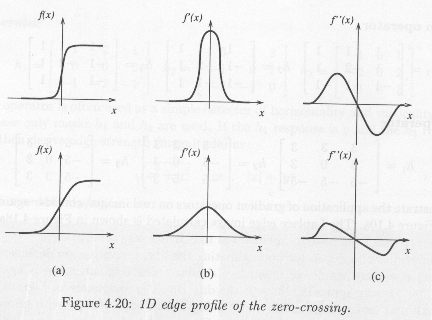
\includegraphics[width=0.6\textwidth]{zero-crossing.png}
  \end{center}
\end{frame}

\begin{frame}
\frametitle{2D Diskrétny prípad}
  \begin{block}{Diskrétny prípad}
  Obraz je diskrétny preto budeme robiť namiesto derivácie diferenciáciu. Teda diskretizovanú verziu derivácie.
  \end{block}

  \begin{block}{2D}
  Obraz je 2-rozmerný a preto použijeme parciálne diferenciálne operátory v rôznych smeroch. 
  \end{block}
\end{frame}

\subsection{Použitie prvej derivácie.}

\begin{frame}
\frametitle{Postup pri použití prvej derivácie}
  \begin{block}{Konvolúcia}
  Diferenciáciu realizujeme pomocou konvolúcie. Matlab má efektívnejšiu implementáciu.
  \end{block}

  \begin{block}{Úloha}
  Pomocou conv2 a prewittovej filtrov nájdite hrany v obrázku zatisie.jpg. Nezabudnite použiť rgb2gray. Keďže máme dva filtre, použite $h = \sqrt{h_x^2 + h_y^2}$ na získanie kombinovaných hrán. Po filtrácii obraz prahujte.
  \end{block}
 
  \begin{block}{Prewittovej filtre}
  \begin{center}
  $\begin{matrix}
    1 & 0 & -1 &    & 1 & 1 & 1 \\
    1 & 0 & -1 & a & 0 & 0 & 0 \\
    1 & 0 & -1 &    & -1 & - 1 & -1
  \end{matrix}$
  \end{center}
  \end{block}
\end{frame}

\begin{frame}
\frametitle{Matlab - edge}
  \begin{block}{edge}
  edge(I, method) - Vráti hranový obraz podľa metódy method. Metódy založené na prvej derivácii sú: 'Sobel', 'Prewitt', 'Roberts' a 'Canny'. Metóda založená na druhej derivácii je 'log', tiež známa ako Marr-Hildrethovej metóda.
  \end{block}
 
  \begin{block}{edge}
  edge(I, method, threshold, direction) - Je možné modifikovať prah po filtrácii a smer filtra.
  \end{block}
\end{frame}

\begin{frame}
\frametitle{Úloha}
  \begin{block}{Úloha}
  Vyskúšajte rôzne hranové detektory založené na prvej derivácii.
  \end{block}
    
  \begin{block}{Šum}
  Detekcia hrán je jeden z algoritmov, ktorý môže značne zlyhať pri prítomosti šumu. Zašumte si obrázok a vyskúšajte na ňom detekovať hrany. Potom skúste odstrániť šum, zlepší sa výsledok?
  \end{block} 
\end{frame}

\begin{frame}
\frametitle{Cannyho detektor}
  \begin{block}{Gaussovo hladenie}
  Cannyho detektor najprv vyhladí obraz pomocou gaussovského filtra.
  \end{block}    
  
  \begin{block}{Non-maximum suppression}
  Po vyhladení sa použije iný detektor využívajúci prvú deriváciu. Keďže jednoduchšie metódy tvoria príliš hrubé hrany v každej oblasti sa zachovajú iba hrany s najsilnejšou odozvou, pritom sa berie do úvahy aj smer hrany.
  \end{block}  
  
  \begin{block}{Slabé a silné hrany}
  Nakoniec sa použijú dva prahy na rozdelenie zvyšných hranových pixelov na dve kategórie: silné a slabé hrany. Silné hrany ostanú vo výsledku. Zo slabých ostanú iba tie ktoré sú napojené na silné hrany, resp. tvoria útvary spolu so silnými hranami.
  \end{block}
\end{frame}

\subsection{Metóda založená na druhej derivácii}

\begin{frame}
\frametitle{Metóda založená na druhej derivácii}
  \begin{block}{Druhá derivácia}
  Hrany môžeme nájsť tam kde druhá derivácia zmení znamienko (funkcia pretne nulu).
  \end{block}
    
  \begin{center}
  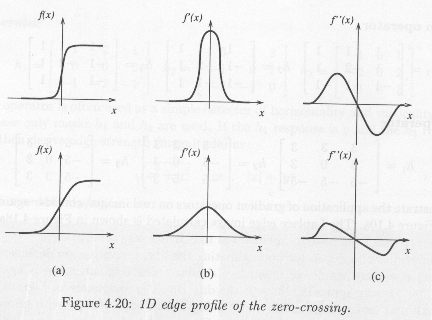
\includegraphics[width=0.6\textwidth]{zero-crossing.png}
  \end{center}
\end{frame}

\begin{frame}
\frametitle{Marr-Hildrethovej metóda}
  \begin{block}{LoG}
  Pre získanie druhej derivácie sa použije Laplacian of Gaussian filter.
  \begin{equation*}
  LoG = -\frac{1}{\pi \sigma^4} \left[ 1 - \frac{x^2 + y^2}{2\sigma^2} \right] e^{-\frac{x^2+y^2}{2\sigma^2}}
  \end{equation*}  
  \end{block}
    
  \begin{center}
  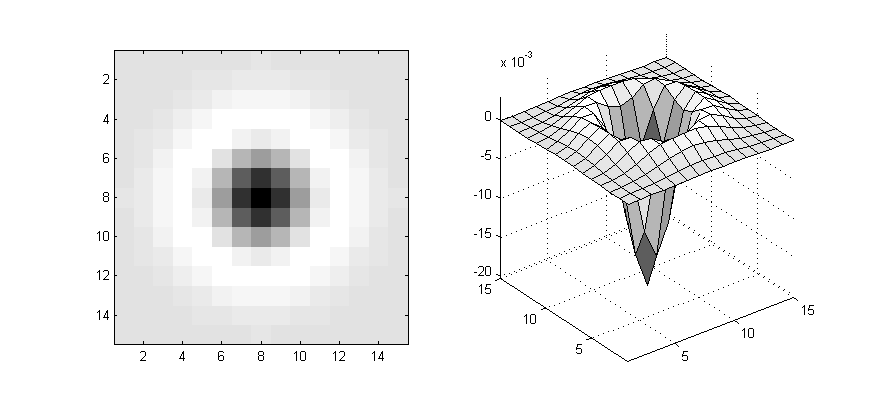
\includegraphics[width=0.8\textwidth]{laplacian_of_gaussian.png}
  \end{center}
\end{frame}

\begin{frame}
\frametitle{Marr-Hildrethovej metóda}
  \begin{block}{Zero-Crossings}
  Po aplikácii druhej derivácie je nutné nájsť body v ktorých sa mení znamienko.
  \end{block}

  \begin{block}{Zrýchlená metóda}
  Dá sa použit aj rozdiel gaussiánov (DoG) namiesto LoG.
  \end{block}   
  
  \begin{block}{Úloha}
  Vyskúšajte Marr-Hildrethovej metódu. V matlabe je pod názvom 'log'.
  \end{block}     
\end{frame}

\section{Ostrenie obrazu}
\subsection{Unsharp Masking}

\begin{frame}
\frametitle{Unsharp masking - Princíp} 
\noindent\makebox[\textwidth]{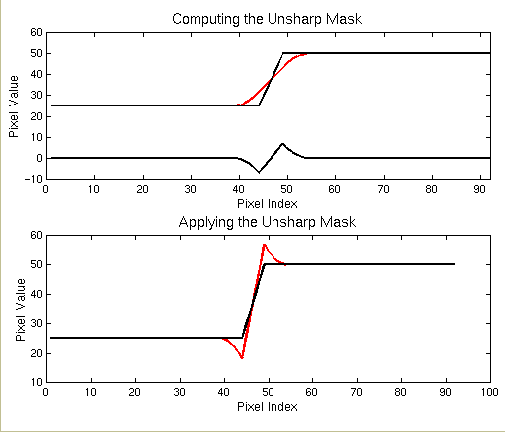
\includegraphics[width=0.9\linewidth]{unsharp.png}}
\end{frame}

\begin{frame}
\frametitle{Unsharp masking} 
  \begin{block}{Unsharp masking}
    Máme obrázok, ktorý je rozostrený. Chceme ho vyostriť. Táto úloha sa dá pochopiť aj ako zvýrazňovanie hrán.
  \end{block} 
 
  \begin{block}{Unsharp masking - princíp}
    $I_{ostr\acute{y}} = I_{origin\acute{a}l} + p \cdot \left( I_{origin\acute{a}l} - I_{vyhladen\acute{y}} \right)$
  \end{block}
  
  \begin{block}{Úloha}
  Vytvorte funkciu unsharp\_mask(I,p,sigma), ktorý aplikuje unsharp masking s parametrom p na obrázok I pomocou gaussovho vyhladenia s hodnotou sigma. Aplikujte na blurred.pgm.
  \end{block}
\end{frame}


\subsection{Laplacián}

\begin{frame}
\frametitle{Laplacián} 
  \begin{block}{Laplacián - definícia}
    $$\Delta f = \nabla \cdot \nabla f = \sum_{i=1}^n \frac{\partial^2 f}{\partial x_i^2} \stackrel{2D}{=} \frac{\partial^2 f}{\partial x^2} + \frac{\partial^2 f}{\partial y^2}$$
  \end{block}
  
  \begin{block}{Konvolučné jadro v 2D}
  $$\begin{bmatrix}
    1 & 1 & 1 \\
    1 & -8 & 1 \\
    1 & 1 & 1 
   \end{bmatrix}
   alebo
   \begin{bmatrix}
    0 & 1 & 0 \\
    1 & -4 & 1 \\
    0 & 1 & 0 
   \end{bmatrix}$$
  \end{block}
    
 \begin{block}{Laplacián v matlabe}
   Generujeme ručne, alebo pomocou fspecial('laplacian',alpha), kde alpha určuje ako veľmi berieme do úvahy diagonálnych susedov.
  \end{block}
\end{frame}

\begin{frame}
\frametitle{Ostrenie pomocou Laplaciánu} 
  \begin{block}{Postup}    
    $I_{ostr\acute{y}} = I_{origin\acute{a}l} - p \left( L_{jadro} \ast I_{origin\acute{a}l}\right)$
  \end{block}

  \begin{block}{Úloha}
  Načítajte obrázok blurred.pgm a použite naň metódu ostrenia pomocou Laplaciánu. Skúste rôzne hodnoty p. Nezabudnite na dátové typy.
  \end{block}
\end{frame}


\end{document}